\chapter{Instalación del framework} \label{sec:instalacion}
En esta sección se describe como instalar el framework en Android Studio; se detallan los requisitos y los pasos a seguir para la instalación.

\section{Requerimientos mínimos:}

\begin{itemize}
\item Android Studio (Java): Si bien esta pensado para y probado en Android Studio, podria funcionar bien en otro entorno que use Java y deje importar archivos Android Archive (.aar).
\item Android SDK API17: Android 4.2 (Jelly Bean) o superior.
\end{itemize}

\section{Pasos para la Instalación:}

\begin{enumerate}
	\item Crear en Android Studio un nuevo proyecto vacío (sin ninguna Activity).
		\begin{itemize}
		\item Seleccionar API17 o superior como versión mínima de Android SDK
		\end{itemize}
		
		
	\item Importar la librería del framework en el proyecto creado:
		\begin{itemize}
		\item Descargar la última versión de \textbf{samplersFramework.aar} desde https://github.com/cientopolis/samplers/releases/
		\item Importar la librería al proyecto: File -$>$ New -$>$ New Module -$>$ Import .JAR/.AAR Package
		\end{itemize}
		
\clearpage		
		
	\item Agregar el repositorio de Google:
	
		En el archivo build.gradle del proyecto agregar: 
\end{enumerate}	
		
\begin{comment}	
\begin{figure}[H]
  \centering
    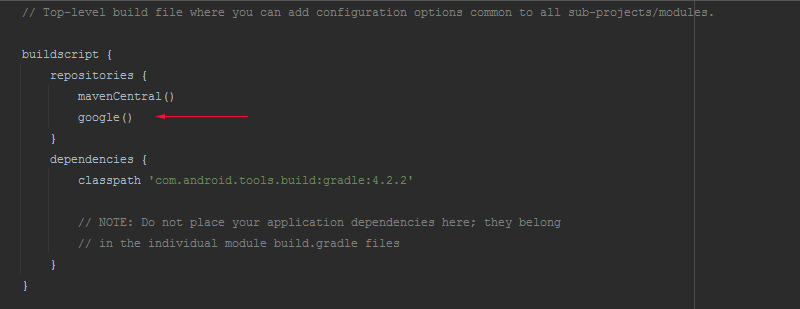
\includegraphics[scale=0.6]{50-anexos/A-instalacion/repositorio_google.png} 
   \caption{Configuración del repositorio de Google}
\end{figure}		
\end{comment}

\begin{lstlisting}[language=Java, frame=tlbr, caption=Configuración del repositorio de Google(línea 4)]
allprojects {
    repositories {
        mavenCentral()
        google()
    }
}
\end{lstlisting}		
							
			
\begin{enumerate}
  \setcounter{enumi}{3}
	\item Agregar las dependencias necesarias:
	
	En el archivo build.gradle de la aplicación agregar: 
	
\end{enumerate}	
	
\begin{comment}	
\begin{figure}[H]
  \centering
    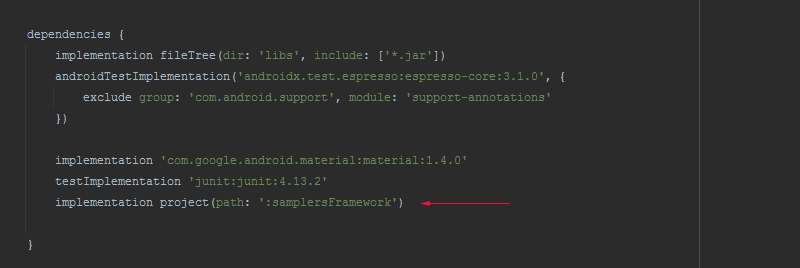
\includegraphics[scale=0.6]{50-anexos/A-instalacion/dependencias.png} 
   \caption{Configuración de las dependencias necesarias}
\end{figure}			
\end{comment}

\begin{lstlisting}[language=XML, frame=tlbr, caption=Configuración de la dependencia del framework (línea 11)]
dependencies {
	implementation fileTree(dir: 'libs', include: ['*.jar'])
	androidTestImplementation('androidx.test.espresso:espresso-core:3.1.0', {
		exclude group: 'com.android.support', module: 'support-annotations'
	})

	implementation 'com.google.android.material:material:1.4.0'
	testImplementation 'junit:junit:4.13.2'

	// agregar la dependencia del framework Samplers
	compile project(":samplersFramework")
}
\end{lstlisting}	
			
			

\begin{enumerate}
  \setcounter{enumi}{4}
	\item Instanciar:

	La instanciación puede ser manual o usando el generador de clases en Gradle como se explicó en la sección \ref{sec:instanciacion}.

\end{enumerate}	





